\section{Background}

% Build up...
In conjunction with increasing performance, memory and storage on modern computers, the capacity for large amounts of varied content in games, movies, and other digital media grows respectively.
However, content creators' capabilities to fully utilize this potential by hand, remains a slow and expensive process.
Because of this, many companies have decided to leverage the use of algorithms in order to create large amounts of rich and varied content.
These algorithms are part of an exciting field within computer science called Procedural Content Generation (PCG).

% What is PCG? (definition)
PCG is a family of algorithms where content such as environments, textures, stories, items, quests, music, weapons, etc.\ is randomly generated rather than designed by hand~\cite[p.1]{PCG_in_games}.
Typically, this is achieved by combining assets and algorithms with computer-generated randomness to synthesize unique content.
However calling it completely random would be incorrect.
The algorithm takes advantage of randomness within its manually defined constraints to generate desired content~\cite{Gamasutra}.
For instance, a PCG algorithm for terrain generation would not construct unreasonable terrain such as lakes flying in the air or trees growing upside down (unless this is intentional).
	
% History and significance
In the early 1980s, PCG was primarily used in games as a work-around for the limited storage space~\cite[p.4]{PCG_in_games}.
In recent years however, the technique has gained a lot of attraction in modern games for generating compelling and replayable experiences.
Games such as Diablo~\cite{diablo} feature procedural generation for the creation of the maps and as well as the placement and number of items and monsters~\cite[p.4]{PCG_in_games}.
In Spore~\cite{spore}~, the animation of the creature the player designs use procedural animation techniques\cite[p.4]{PCG_in_games}.
Furthermore, the popular game Minecraft~\cite{minecraft} make use of PCG techniques extensively for generating everything from the cave-systems to the mountains to the whole world~\cite[p.4]{PCG_in_games}.
Procedural generation can be used to generate pretty much any virtual content you could imagine.
Evident from the use of PCG in big commercial games there is a demand from the game industry to create large, impressive and unique environments for their player base to explore.

% More specific games


\subsection{Theory}

\subsubsection{Noise}

One of the most fundamental tools used in PCG is noise.
Noise is the concept of random values, often represented using a 2D or 3D matrix of real numbers.
The two major types of noise that are commonly used are \textit{value noise} and \textit{gradient noise}.

\textit{Value noise} is constructed by first randomizing the values of a few lattice points in the matrix, and then interpolating these values for intermediate points.
Bilinear and bicubic interpolation are common in practice since they are fast to compute.
Value noise is simple to implement, but it has several disadvantages.
First off, the noise ends up with a grid-like structure because of the lattice points.
This is often undesired since it creates arbitrary patterns in the noise.
Furthermore, neighboring lattice points may greatly differ in values which can result in sudden changes in steepness.

\newpage
\textit{Gradient noise} solves the problems with value noise by first constructing slopes, and then sample values from those.
By interpolating slopes (or gradients) that already are smooth, we ensure that not only changes in values are smooth but also the \textit{rate of change} between them.
This causes nearby points to be of similar random values, while points far apart to be unrelated.

Both types of noise can be represented with intensity maps as seen in figure~\ref{fig:noisetypes}.
An intensity map is a bitmap image where each pixel represents the value of the underlying noise.
White pixels indicate maximum values, and black pixels represent minimum values.
These maps can be used to represent many things including heights, in which case they are referred to as \textit{heightmaps}.
They can also be used to create a smooth blending between textures.

\begin{figure}[h!]
  \centering
  \begin{subfigure}[b]{0.30\textwidth}
    \frame{
\includegraphics[width=\textwidth]{figure/value_noise.png}}
    \caption{Value noise. \cite{value_noise}}
  \end{subfigure}
  \quad
  \quad
  \quad
  % NOTE(anton): image generated from https://cpetry.github.io/TextureGenerator-Online/
  \begin{subfigure}[b]{0.30\textwidth}
    \frame{
\includegraphics[width=\textwidth]{figure/heightmap.png}}
    \caption{Gradient noise.}
  \end{subfigure}

  \caption{Examples of value noise and gradient noise represented using intensity maps. Notice how the value noise has cross-like patterns.}
  \label{fig:noisetypes}
\end{figure}

A commonly used implementation of gradient noise is \textit{Perlin noise}, which later evolved into an improved version called \textit{simplex noise}.
Ken Perlin introduced \textit{Perlin noise} in 1985 intending to produce more natural-looking textures \cite{perlin_noise}.
Although \textit{simplex noise} is the improved version, the two terms are often used interchangeably. The idea of \textit{simplex noise} is described in great detail by Stefan Gustavson in his paper \textit{Simplex noise demystified} \cite{simplex_noise}.
He also mentions several technical advantages with the technique.
This subsection describes different ways of generating procedural content, for example, Gradient noise and L-systems.

\subsubsection{Search-based}
One method for generating content is using a \textit{search-based} approach.
This often involves using an evolutionary algorithm with some stochastic search/optimization algorithms to determine a solution with desired qualities.
The general idea is that for a given design problem we can find an acceptable solution by ``searching'' for it within the solution space.
Solutions are iterated and then tweaked according to an evaluation function that keeps the changes that make the solution(s) ``better'' and discards any harmful changes.
By iterating and tweaking one or many of possible solutions we will eventually arrive at the desired solution.

\subsubsection{Machine Learning}
Machine Learning (ML) is another method that can be used to procedurally generate content.
The idea with this technique is to generate new content based patterns found from analyzing existing content.
This technique can prove to be especially useful when it is hard to explicitly define the content that should be generated.
For instance, it is easier to analyze and replicate the design of existing cities as opposed to manually defining what a ``good'' city is.
The catch is that a lot of well-structured data is needed to draw these statistical conclusions.

Summerville et al. refers to this synergy between ML and PCG as \textit{PCGML} (PCG via ML)~\cite{lmao_ml}.
They also contribute with several interesting insights to this relatively unexplored field such as the use of Unsupervised Learning.
This field is quite extensive and might need considerably more research in the case that ML will be utilized.

\subsubsection{Voronoi Diagram}
Voronoi diagram can be used to divide an area into subareas that look more natural than a normal grid. 
The construction of the diagram starts with a number of points inside the area, either given by a user or randomly plotted. 

These points are the black dots that can be seen in the diagrams in figure \ref{fig:voronoi}.
Each of these black dots represents different subareas, which are represented as different colors in the same figure.
Each point inside the area is then associated with the subarea of the black dot that is closest.

\begin{figure}[H]
  \centering
  \begin{subfigure}[b]{0.49\textwidth}
    \frame{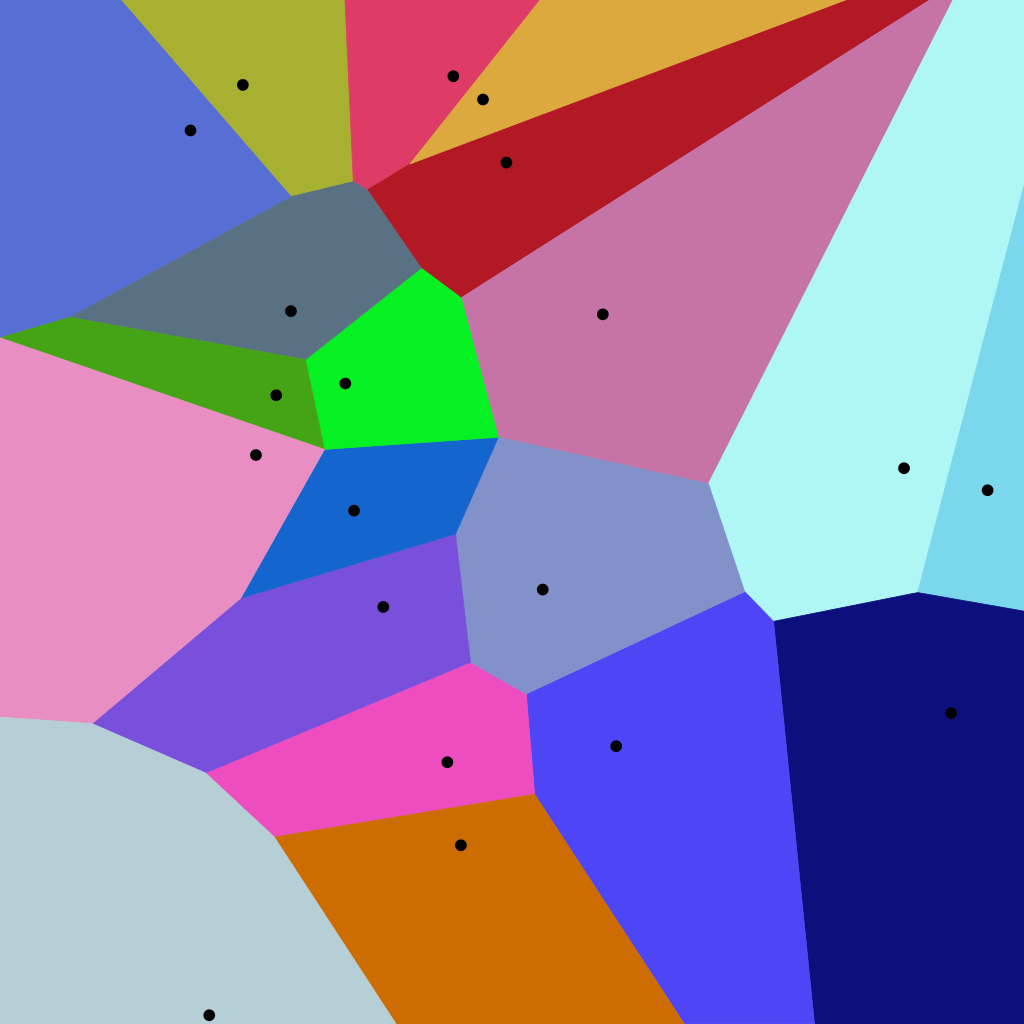
\includegraphics[width=\linewidth]{figure/Euclidean_Voronoi_diagram.png}}
    \caption{Voronoi diagram using Euclidean distance \cite{voronoi_diagram_euclidean}.}
    \label{fig:voronoi_euclidean}
  \end{subfigure}
  \begin{subfigure}[b]{0.49\textwidth}
    \frame{
\includegraphics[width=\linewidth]{figure/Manhattan_Voronoi_Diagram.png}}
    \caption{Voronoi diagram using Manhattan distance \cite{voronoi_diagram_manhattan}.}
    \label{fig:voronoi_manhattan}
  \end{subfigure}
  \caption{Voronoi diagrams with two different ways of associating each point to a position within an area.}
  \label{fig:voronoi}
\end{figure}

\subsubsection{L-System}
An L-system is a type of formal grammar typically used in procedural generation.
It is built up of strings which under a set of constraints recursively grow larger and more complex with each iteration.
These strings are then used to build geometric structures.
L-system grammars are defined by three parameters which can be denoted as follows:

\begin{itemize}
  \item V  - The alphabet, consists of symbols that are referred to as constants or variables.
  \item $\omega$ - an axiom, an initial symbol from V which defines the initial state of the system.
  \item P - Production rules, these are the constraints which determine how variables should be replaced.
\end{itemize}

The variables are replaced with a mix of variables and constants, which recursively leads to a very large and complex resulting set.
One special attribute of L-systems is that rather than the constants and variables being evaluated one by one in a left to the right manner they are all evaluated in parallel.

A special case of L-systems is referred to as \textit{Stochastic bracketed L-systems}.
A grammar being stochastic means that there are some production rules which can be applied to each variable that all have a different probability of occurring.
Bracketed means that we have a push/pop structure where a \textbf{[} means that we push a value, storing it, and a \textbf{]} means that we return to where we pushed most recently.
By being able to return to a previous state, one can produce content with less continuous generation.
This is well expressed in the book Procedural Content Generation in Games~\cite[p.77]{PCG_in_games}, where they describe the limitations of non-bracketed L-systems in the following way:
“While interpreting L-system-generated strings as turtle instructions allow us to draw complex fractal shapes, we are fundamentally limited by the constraint that the figures must be drawable in one continuous line—the whole shape must be drawn “without lifting the pencil””. 

\subsubsection{Poisson Disc Sampling}

This algorithm randomizes the placement of points such that they are close to each other, but not closer than a specified distance.
The idea is to specify a distance $R$ and then place a single \textit{active} point in a random position.
While there are \textit{active points} left, we pick some active points and attempt to place points within a distance $[R, 2R]$.
Placed points may not be closer than $R$ distance to any other point, and when no new points can be placed from an active point, we mark that active point as \textit{inactive}.
A previous BA project utilized this technique with successful results \cite{ba_landscape}.
\section{Related Works}

Generation of cities has been an active area of research for almost 20 years by now, with the \textit{Procedural Modeling of Cities} paper by Müller et al. being the pioneer \cite{muller_city_gen}.
This paper outlines the \textit{CityEngine} system, which makes heavy use of L-systems (see Chapter \ref{chap:lsystem}) to generate Manhattan-style cities from various image maps as input.
The system produces impressive results, and the paper itself proposes many interesting ideas that extend beyond L-systems.
\textit{CityEngine} later evolved into a commercial application \cite{esri}, demonstrating the real-life potential of this type of software.
Unfortunately, \textit{CityEngine} is quite expensive and remains closed-source.
Nonetheless, the original paper has been a major inspiration for our work.

Kelly and McCabe have also made significant contributions to this field with the development of \textit{Citygen} \cite{citygen_paper}, and the conduction of a prestudy \cite{citygen_paper_prestudy} summarizing common city generation techniques. 
\textit{Citygen} is an interactive system where users model cities in real-time, being heavily assisted and accelerated with the use of PCG techniques.
The paper emphasizes road generation and lot subdivision, detailing several intriguing concepts such as road graph hierarchy, snap algorithms for road segments, and strategies for building roads between significant elevation differences.

A tendency found amongst early work on road generation is that L-systems have frequently been used.
Another common approach has been agent-based generation \cite{agent_based_roads}, especially in more recent work \cite{tmwhere} \cite{robin}.
Recently, there have also been some experimentation done using the WaveFunctionCollapse (WFC) algorithm \cite{wavefunc} to generate roads \cite{wavefunc_roads}.
However, it remains difficult to determine WFC's potential compared to previous approaches as more research needs to be done \cite[p.50]{wavefunc_roads}.

Outside of academia, there has also been promising work done related to city generation.
A decade-old tech demo from \textit{Introversion Software} shows a promising generation of the outline of a city, complete with a graphical interface \cite{subversion}.
The \textit{SceneCity} plugin for Blender \cite{blender} is able to produce highly detailed buildings connected by grid-based roads \cite{scenecity}.
Impressive PCG cities can also be found in modern games such as \textit{Marvel's Spider-Man} \cite{pcg_spiderman} and \textit{The Sinking City} \cite{pcg_sunken_city}.

Unfortunately, most progress towards city generation so far remains closed-source and behind paywalls.
Exceptions exist but tend to be deprecated or incomplete solutions.
Our contribution aims to deviate from this by being open-source, free, and able to generate cities complete with terrain, roads, and buildings.
With this, we believe that the progress of city generation will be more accessible to industry and academia alike.
Accordingly, ideas presented in previous work will be combined in various ways to produce a complete, standalone city generation software.

% Benefits
% A key question to consider is what the actual benefits are of using PCG over manual design is.
% With the help of PCG, software can produce impressive, varied and seemingly endless environments order of magnitudes faster than a human~\cite[p.3]{PCG_in_games}.
% This aids designers to create a lot more content cheaply and efficiently once the algorithm has been developed.
% Additionally, as soon as the algorithm is done it can be reused. Similar to a debugger, a PCG algorithm can be infinitely run afterwards. The algorithm can potentially be reused to generate completely different content from.

% Although the output space of PCG is considerable, automatic content generation comes with a set of obstacles.
% One of the challenges when developing PCG systems is the ability to generate content comparable with the quality of hand-crafted content.
% In the case of hand-crafted content, the content would undoubtedly fit its intended use case whereas generated content might be deemed inadequate or specific enough.
% This difficulty also ties into the problem of generating visually distinctive and expressive content.
% If the generated content only differs with minimal variance it might not actually be perceived as varied content at all as
% the computed creativity PCG offers has its limits. For instance, there are no reasonable automatic novel creators. Kate Compton, who is a programmer that worked on Spore's and SimCity's content generation, had a presentation about the utilities that PCG offers. She mentions that writing a novel is too general of a task for PCG to generate, and that PCG excells to generate very specifically defined~\cite{PCG_for_everyone}. Although it is technically possible it would not compare well to human novel writing.